\documentclass[language={english},style=solution]{smo}

\title{%
    \de{Zweite Runde 2021}%
    \fr{Deuxième tour 2021}%
    \en{Second round 2021}%
}
\examdate{%
    \de{19. Dezember 2020}%
    \fr{19 décembre 2020}% 
    \en{19 December 2020}%
}
\examplace{%
    \de{Lausanne, Lugano, Zürich}%
    \fr{Lausanne, Lugano, Zurich}%
    \en{Lausanne, Lugano, Zürich}%
}

\begin{document}

\de{Eine vollständige Lösung ist 7 Punkte wert. Bei jeder Aufgabe kann es bis zu 2 Punkte Abzug geben für kleine Fehler bei einer sonst korrekten Lösung. Teilpunkte werden gemäss dem Punkteschema vergeben.

Im Anschluss befinden sich die Lösungen mit Vorrundentheorie, die den Korrektoren bekannt sind. Am Ende jedes Problems werden noch alternative Lösungen präsentiert, die auch andere Theorie verwenden können. Während des Trainings zu Hause werden die Teilnehmenden dazu ermutigt, alle ihnen bekannten Methoden zu verwenden. An der Prüfung hingegen ist es nicht empfohlen mit Methoden, welche sie unter Prüfungskonditionen nicht genügend beherrschen, nach alternativen Lösungen zu suchen. Damit wird riskiert, dass wertvolle Zeit verloren geht.}

\fr{\textbf{Remarque liminaire:} Une solution complète rapporte 7 points. Pour chaque problème, jusqu'à 2 points pourront être déduits d'une solution correcte en cas de lacunes mineures. Les solutions partielles sont évaluées selon le barème suivant.

Ci-dessous vous trouverez les solutions élémentaires connues des correcteurs. Des solutions alternatives sont présentées à la fin de chaque problème. Les étudiants sont naturellement encouragés à essayer toutes les méthodes à leur disposition lors de l'entrainement, mais sont également avisés de ne pas chercher de solutions alternatives qui emploient des méthodes qu'ils ne maîtirent pas en condition d'examen, au risque de perdre un temps précieux.}

\en{\textbf{Preliminary remark:} A complete solution is worth 7 points. For every problem, up to 2 points can be deducted from a correct solution for (minor) flaws. Partial marks are attributed according to the marking schemes.

Below you will find the elementary solutions known to correctors. Alternative solutions are presented in a complementary section at the end of each problem. Students are encouraged to use any methods at their disposal when training at home, but should be wary of attempting to find alternative solutions using methods they do not feel comfortable with under exam conditions as they risk losing valuable time.}

\begin{enumerate}

\item[\textbf{G1)}]
\de{Sei $k$ ein Kreis mit Mittelpunkt $O$. Seien $A$, $B$, $C$ und $D$ vier unterschiedliche Punkte auf dem Kreis $k$ in dieser Reihenfolge, sodass $AB$ ein Durchmesser von $k$ ist. Der Umkreis des Dreiecks $COD$ schneide $AC$ zum zweiten mal in $P$. Zeige, dass $OP$ und $BD$ parallel sind.

\textbf{Lösung 1 (Louis), Winkeljagd:} 
Wir zeigen, dass $\angle ODB=\angle POD$. Dies beweist, dass die Linien parallel sind.

Da $O$ der Mittelpunkt des Kreises ist, haben wir $OD=OB$ und somit ist das Dreieck $ODB$ gleichschenklig an $O$. Somit ist $\angle ODB = \angle OBD$. Weil $O$ auf der Strecke $AB$ liegt, wissen wir $\angle OBD=\angle ABD$. Die Punkte $A,B,C,D$ sind auf einem Kreis, also $\angle ABD=\angle ACD=\angle PCD$. Zum Schluss sind die Punkte $C,O,D,P$ alle auf einem Kreis und $\angle PCD=\angle POD$. Also haben wir
\[
\angle ODB=\angle POD.
\]
und wir sind fertig.

\textbf{Marking Scheme}

Für unvollständige Lösungen sind folgende Punkte möglich. ($\leq$ 4P):
\begin{enumerate}
    \item Working Forward Punkte:
    
    \textbf{Bemerkung:} Für die folgenden Winkelgleichungen sind Markierungen auf der Skizze \textbf{nicht} ausreichend. Die Beziehungen sollten anderswo explizit genannt werden.
    \begin{itemize}
        \item +1P: Eine Winkelbeziehung im Sehnenviereck $ABCD$ \textbf{oder} $CPDO$ finden (zB. $\angle PCD=\angle POD$ oder $\angle DBA=\angle ACD$)
        \item +1P: Eine Winkelbeziehung zwischen den beiden Sehnenvierecken $ABCD$ \textbf{und} $CPDO$ finden (zB. $\angle PCD=\angle DBA$)
        \item +1P: Eine Winkelbeziehung finden, welche benutzt, dass $O$ der Mittelpunkt des Kreises um $ABCD$ ist (zB. $\angle ODB=\angle OBD$)
    \end{itemize}

    \item Working Backward Punkte:
    \begin{itemize}
        \item +1P: Die gewünschte Bedingung mit Winkeln ausdrücken  (zB. $\angle POD=\angle ODB$ oder $\angle DBA=\angle POA$)
    \end{itemize}
\end{enumerate}
}

\fr{Soit $k$ un cercle de centre $O$. Soient $A$, $B$, $C$ et $D$ quatre points distincts sur $k$, dans cet ordre, tels que $AB$ est un diamètre de $k$. Le cercle circonscrit au triangle $COD$ intersecte $AC$ une deuxième fois en $P$. Montrer que $OP$ et $BD$ sont parallèles.

\textbf{Solution 1 (Louis), Chasse aux angles:}

On va montrer que $\angle ODB=\angle POD$. Cela prouve que les droites sont parallèles.

Comme $O$ est le centre du cercle, on a $OD=OB$ et donc le triangle $ODB$ est isocèle en $O$. Donc $\angle ODB = \angle OBD$. Comme $O$
se trouve sur le segment $AB$, $\angle OBD=\angle ABD$. Les points $A,B,C,D$ étant sur un même cercle, on a $\angle ABD=180^\circ-\angle ACD=\angle PCD$. Finalement, les points $C,O,D,P$ se trouvent sur un même cercle et donc $\angle PCD=\angle POD$. On a donc bien
\[
\angle ODB=\angle POD.
\]

\textbf{Marking Scheme}

Pour les solutions partielles, on attribuera les points additifs suivants ($\leq$ 4P):
\begin{enumerate}
    \item Forward points:
    
    \textbf{Remarque:} Pour les relations d'angles qui suivent, des angles bien marqués sur un dessin propre \textbf{ne sont pas} suffisants. Les relations doivent se trouver explicitement ailleurs.
    \begin{itemize}
        \item +1P: établir une relation d'angles dans les quadrilatères inscrits $ABCD$ \textbf{ou} $CPDO$ (eg. $\angle PCD=\angle POD$ ou $\angle DBA=\angle ACD$)
        \item +1P: établir une relation d'angles en combinant les quadrilatères inscrits $ABCD$ \textbf{et} $CPDO$ (eg. $\angle PCD=\angle DBA$)
        \item +1P: établir une relation d'angle en utilisant que $O$ est le centre du cercle $ABCD$ (eg. $\angle ODB=\angle OBD$)
    \end{itemize}

    \item Backward points:
    \begin{itemize}
        \item +1P: reformuler la conclusion en termes d'angles (eg. $\angle POD=\angle ODB$ ou $\angle DBA=\angle POA$)
    \end{itemize}
\end{enumerate}
}

\ita{}

\en{
Let $k$ be a circle with center $O$. Let $A$, $B$, $C$ and $D$ be four distinct points on $k$ in this order such that $AB$ is a diameter of $k$. The circumcircle of the triangle $COD$ intersects $AC$ again in $P$. Show that $OP$ and $BD$ are parallel.

\textbf{Solution 1 (Louis), Angle chasing:} 
We will show that $\angle ODB=\angle POD$, which proves that the lines are parallel.

As $O$ is the centre of the circle, we have that $OD=OB$ and so the triangle $ODB$ is isoceles in $O$. So $\angle ODB = \angle OBD$. As $O$ lies on the segment $AB$, $\angle OBD=\angle ABD$. The points $A,B,C,D$ are concyclic so we also have $\angle ABD=\angle ACD=\angle PCD$. Finally, the points $C,O,D,P$ are all on a circle and so $\angle PCD=\angle POD$. Therefore, we have
\[
\angle ODB=\angle POD.
\]
and we are done.

\textbf{Marking Scheme}

For partial solutions, the following points are available ($\leq$ 4P):
\begin{enumerate}
    \item Forward points:
    
    \textbf{Remark:} For the following angle equalities, angles marked on a drawing \textbf{are not} sufficient. The relation should be explicitly stated elsewhere.
    \begin{itemize}
        \item +1P: establish an angle equality in the cyclic quadrilaterals $ABCD$ \textbf{or} $CPDO$ (eg. $\angle PCD=\angle POD$ or $\angle DBA=\angle ACD$)
        \item +1P: establish an angle equality combining the two quadrilaterals $ABCD$ \textbf{and} $CPDO$ (eg. $\angle PCD=\angle DBA$)
        \item +1P: establish an angle qualitiy using that $O$ is the centre of the circle $ABCD$ (eg. $\angle ODB=\angle OBD$)
    \end{itemize}

    \item Backward points:
    \begin{itemize}
        \item +1P: reformulate the conclusion in terms of angles (eg. $\angle POD=\angle ODB$ or $\angle DBA=\angle POA$)
    \end{itemize}
\end{enumerate}
}


\newpage

\textbf{Alternative solutions}

\textbf{Solution 2 (Tanish), Nine-point circle:} 

Let $X$ be $AC \cap BD$ and $Q$ be the second intersection of $BD$ and $(COD)$. We will prove that $(COD)$ is the nine-point circle of $AXB$. But this is clear - $O$ is the midpoint of $AB$, $D$ is the base of the altitude dropped from $B$ (Thales) and $C$ is the base of the altitude dropped from $A$ (Thales). It follows that $P$ and $Q$ are the midpoints of $AX$ and $BX$ respectively, and $XPOQ$ is a parallelogram.

\textbf{Solution 3 (Tanish), Inversion:}

Let us invert about $k$. $AC$ is sent to the circumcircle of $OAC$; the circumcircle of $OAD$ is sent to $DC$. This means that $P'$ is the intersection of these two. $OP$ is sent to the line $OP'$ and $BC$ is sent to $BC$, so it suffices to prove that $OP' \parallel BD$. This is equivalent to $\angle AOP' = \angle ABD$. Since $\angle ABD = 2\angle AOD$, we simply have to prove $OP'$ bisects $\angle AOD$, or that (as $AO = OD$), $OP'$ bisects $\angle AP'D.$ However this last statement is clearly true when you consider the circumcircle of $AODP'$ as $\angle OP'A$ subtends the arc $\overset{\frown}{OA}$ and $\angle OP'D$ subtends the arc $\overset{\frown}{OC}$, which are of equal length as $OA = OC$. \newline \newline
\emph{Note}: $OP$ is the same line as $OP'$ and therefore you could equally prove that $OP$ bisects $AOD$ or $APD$, but this is not as trivial.
\newpage

\item[\textbf{G2)}]
\en{Let $ABC$ be an acute triangle with $BC > AC$. The perpendicular bisector of the segment $AB$ intersects the line $BC$ at $X$ and the line $AC$ at $Y$. Let $P$ be the projection of $X$ on $AC$ and let $Q$ be the projection of $Y$ on $BC$. Prove that the line $PQ$ intersects the segment $AB$ at its midpoint.

\textbf{Solution 1 (angle chasing, cylic quadrilaterals):} Introducing $M$ as the midpoint of $AB$, the exercise is equivalent to showing that $M$, $P$ and $Q$ are collinear. In order to do that, we will show that $\angle MPX+\angle XPQ=180^\circ$. We first note that there are a few cyclic quadrilaterals :
\begin{enumerate}
    \item $YQPX$ is cyclic, as $\angle XPY=90^\circ=\angle XQY$.
    \item $YQMB$ is cyclic, as $\angle BMY=90^\circ=\angle BQY$.
    \item $AMXP$ is cylic, as $\angle XMA=90^\circ=\angle XPA$.
\end{enumerate}
As $X$ is on the perpendicular bisector of $AB$, we have $XA=XB$ and $\angle MAX=\angle MBX\;(*)$.

Then,
\[
    \angle MPX\stackrel{\text{(c)}}{=} \angle MAX
    \stackrel{(*)}{=} \angle MBX
    = \angle MBQ
    \stackrel{\text{(b)}}{=} \angle MYQ
    = \angle XYQ
    \stackrel{\text{(a)}}{=} 180^\circ - \angle XPQ.
\]

\textbf{Solution 2 (more efficient than Solution 1):} There is a very similar way way to proceed, making use of only two of the aforementioned cyclic quadrilaterals, and that $YA=YB$ implies $\angle MYA=\angle MYB\;(*)$. This time, we show that $M$, $P$ and $Q$ are collinear by proving that $\angle XQP=\angle XQM$. Indeed,
\[
\angle XQP\stackrel{\text{(a)}}{=}\angle XYP=\angle MYA\stackrel{(*)}{=}\angle MYB\stackrel{\text{(b)}}{=}\angle MQB=\angle XQM.
\]

\textbf{Solution 3 (Menelaus and power of a point):} One could be tempted to show that $M$, $P$ and $Q$ are collinear by using Menelaus. We would need to prove that 
\[
\frac{AM}{MB}\cdot \frac{BQ}{QC}\cdot \frac{CP}{PA}\stackrel{?}{=}-1.
\]
Firstly, like in the other proofs, we note that $YQPX$ is cyclic as $\angle XPY=90^\circ=\angle XQY$. We will write $\omega$ for the circle $(YQPX)$. By Thales on a circle, its center is the midpoint of $XY$, in particular it lies on the perpendicular bisector of $AB$. As the power of a point with respect to $\omega$ is uniquely determined by its distance to this center, we have that $A$ and $B$ have the same power with respect to $\omega$, proving that 
\[
PA\cdot AY=XB\cdot BQ.
\]
The power of $C$ with respect to $\omega$ also yields that
\[
CX\cdot QC=CP\cdot YC.
\]
Combining these two equalities, we finally have that
\[
\frac{AM}{MB}\cdot \frac{BQ}{QC}\cdot \frac{CP}{PA}=-1\cdot \frac{BQ}{PA}\cdot \frac{CP}{QC}=-1\cdot \frac{AY}{XB}\cdot \frac{CX}{YC} =\frac{BM}{MA}\cdot \frac{AY}{YC}\cdot \frac{CX}{XB}=-1.
\]
In the last equality, we used Menelaus as $M$, $Y$ and $X$ are collinear.
\begin{center}
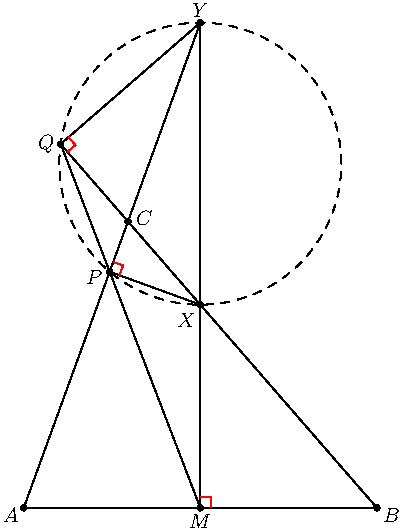
\includegraphics{g2fig}
\end{center}

\bigskip

\textbf{Marking Scheme - Solution 1 and 2}

\begin{itemize}
    \item 1P: Rewriting the statement in terms of angles, in a statement of the kind : 
    \begin{itemize}
        \item $\angle MPX+\angle XPQ=180^\circ$
        \item $\angle XQP=\angle XQM$
    \end{itemize}
    \item 3P: Showing that $YQPX$, $YQMB$ or $AMXP$ are cyclic (2P for one quadrilateral, 3P for two or three quadrilaterals)
    \item 1P: Proving that $\angle MAX=\angle MBX$, $\angle MAY=\angle MBY$ or that $\angle MYA=\angle MYB$.
    \item 2P: Conclude.
\end{itemize}

\textbf{Marking Scheme - Solution 3}

\begin{itemize}
    \item 1P: Stating the problem as a Menelaus equality.
    \item 1P: Proving that $YQPX$ is cyclic.
    \item 2P: Proving that $PA\cdot AY=XB\cdot BQ$.
    \item 1P: Proving that $CX\cdot QC=CP\cdot YC$.
    \item 2P: Conclude.
\end{itemize}
}

\de{Sei $ABC$ ein spitzwinkliges Dreieck mit $BC > AC$. Die Mittelsenkrechte der Seite $AB$ schneidet die Gerade $BC$ in $X$ und die Gerade $AC$ in $Y$. Sei $P$ die Projektion von $X$ auf $AC$ und sei $Q$ die Projektion von $Y$ auf $BC$. Beweise, dass die Gerade $PQ$ die Strecke $AB$ in ihrem Mittelpunkt schneidet.

\textbf{Lösung 1 (Winkeljagd, Sehnevierecke):}
Nach einführung von $M$ als der Mitpunkt von $AB$, genügt es zu zeigen, dass $P$, $Q$ und $M$ kolinear sind. Wir werden dies hier zeigen, indem wir beweisen, dass $\angle MPx + \angle XPQ = 180^\circ$ gilt.
Wir bemerken sazu zuerst ein paar Sehenenvierecke.
\begin{enumerate}
    \item $YQPX$ ist ein Sehnenviereck, da $\angle XPY = 90^\circ = \angle XQY$.
    \item $YQMB$ ist ein Sehnenviereck, da $\angle BMY = 90^\circ = \angle BQY$.
    \item $AMXP$ ist ein Sehnenviereck, da $\angle XMA = 90^\circ = \angle XPA$.
\end{enumerate}
Da nun $X$ auf der Mittelsenkrechten von $AB$ liegt, gilt $XA = XB$ und somit $\angle MAX = \angle MBX \;(*)$
Alles in allem gilt also:
\[
    \angle MPX\stackrel{\text{(c)}}{=} \angle MAX
    \stackrel{(*)}{=} \angle MBX
    = \angle MBQ
    \stackrel{\text{(b)}}{=} \angle MYQ
    = \angle XYQ
    \stackrel{\text{(a)}}{=} 180^\circ - \angle XPQ.
\]
Wie gewünscht.

\textbf{Lösung 2 (effizienter als Lösung 1):} Es gibt eine sehr ähnliche Vorgehensweis, die nur zwei der zuvorgenannten Sehnenvierecke benützt. Ebenfalls benutzen wir, dass $YA = YB$ bzw. $\angle MYA = MYB\;(*)$. Dieses Mal werden wir zeigen, dass $M$, $P$ und $Q$ kolinear sind, indem wir zeigen, dass $\angle XQP = XQM$. Wieder mit den obig genannten Sehnenvierecken gilt:

\[
\angle XQP\stackrel{\text{(a)}}{=}\angle XYP=\angle MYA\stackrel{(*)}{=}\angle MYB\stackrel{\text{(b)}}{=}\angle MQB=\angle XQM.
\]
Wie gewünscht.

\textbf{Lösung 3 (Menelaus und Potenz eines Punktes):} Man kann die kolinearität auch mit Menelaus zeigen. Dazu müsste man die folgende Gleichung verifizieren:
\[
\frac{AM}{MB}\cdot \frac{BQ}{QC}\cdot \frac{CP}{PA}\stackrel{?}{=}-1.
\]
Wie in den anderen beiden Lösungen, bemerken wir, dass $YQPX$ ein Sehnenviereck ist, da $\angle XPY = 90^\circ = \angle XQY$. Wir werden nun $\omega$ für den Kreis $(YQPX)$ schreiben. Nach dem Satz von Thales ist das Zentrum von $\omega$ der Mittelpunkt von $XY$, also vorallem auch auf der Mittelsenkrechten zu $AB$. Da die Potenz eines Punktes nur von der Distantz zum Kreismittelpunkt abhängt, ist die Potenz von $A$ und $B$ gleich bezüglich $\omega$, woraus folgt:
\[
PA\cdot AY=XB\cdot BQ.
\]
Betrachtet man auch noch die Potenz des Punktes $C$ erhält man
\[
CX\cdot QC=CP\cdot YC.
\]
Die beide Gleichungen zusammen ergeben nun
\[
\frac{AM}{MB}\cdot \frac{BQ}{QC}\cdot \frac{CP}{PA}=-1\cdot \frac{BQ}{PA}\cdot \frac{CP}{QC}=-1\cdot \frac{AY}{XB}\cdot \frac{CX}{YC} =\frac{BM}{MA}\cdot \frac{AY}{YC}\cdot \frac{CX}{XB}=-1.
\]
Wobei wir in der letzten Gleichung Menalaus auf $ABC$ und die Tatsache, dass $M$, $Y$ und $X$ kolinear sind, benutzt haben.

\begin{center}
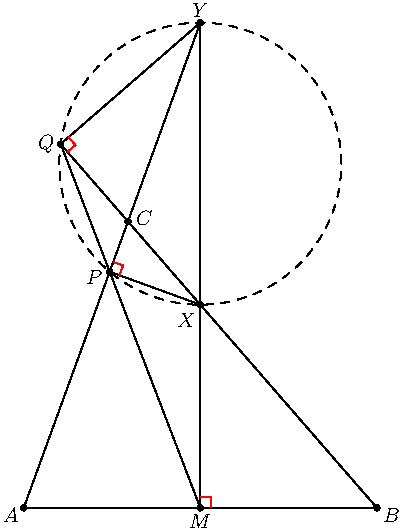
\includegraphics{g2fig}
\end{center}

\bigskip

\textbf{Marking Scheme - Lösung 1 und 2}
\begin{itemize}
    \item 1P: Umschreibung der zu beweisenden Aussage mit einer Winkelgleichung, wie beispielsweise:
    \begin{itemize}
        \item $\angle MPX+\angle XPQ=180^\circ$
        \item $\angle XQP=\angle XQM$
    \end{itemize}
    \item 3P: Zeigen, dass $YQPX$, $YQMB$ oder $AMXP$ Sehnenvierecke sind (2P für ein Sehenviereck, 3P für zwei oder drei Sehnenvierecke)
    \item 1P: Zeigen, dass $\angle MAX=\angle MBX$, $\angle MAY=\angle MBY$ oder dass $\angle MYA=\angle MYB$
    \item 2P: Den Beweis vollenden
\end{itemize}

\textbf{Marking Scheme - Lösung 3}

\begin{itemize}
    \item 1P: Das Problem zu einer Menelaus Gleichung umformen
    \item 1P: Zeigen, dass $YQPX$ zyklisch ist
    \item 2P: Zeigen, dass $PA\cdot AY=XB\cdot BQ$
    \item 1P: Zeigen, dass $CX\cdot QC=CP\cdot YC$
    \item 2P: Den Beweis vollenden
\end{itemize}
}




%french
\fr{Soit $ABC$ un triangle aigu avec $BC > AC$. La médiatrice du segment $AB$ coupe la droite $BC$ en $X$ et la droite $AC$ en $Y$. Soient $P$ la projection de $X$ sur $AC$ et $Q$ la projection de $Y$ sur $BC$. Montrer que la droite $PQ$ coupe le segment $AB$ en son milieu.

\textbf{Solution 1 (chasse aux angles, quadrilatères cycliques):} En posant $M$ comme le milieu d'$AB$, l'exercice est équivalent à montrer que $M$, $P$ et $Q$ sont colinéaires. Pour faire cela, nous allons montrer que $\angle MPX+\angle XPQ=180^\circ$. Nous notons d'abord qu'il y a quelques quadrilatères cycliques :
\begin{enumerate}
    \item $YQPX$ est cyclique, car $\angle XPY=90^\circ=\angle XQY$.
    \item $YQMB$ est cyclique, car $\angle BMY=90^\circ=\angle BQY$.
    \item $AMXP$ est cyclique, car $\angle XMA=90^\circ=\angle XPA$.
\end{enumerate}
Comme $X$ est sur la médiatrice d'$AB$, nous avons $XA=XB$ et $\angle MAX=\angle MBX\;(*)$.

Alors,
\[
    \angle MPX\stackrel{\text{(c)}}{=} \angle MAX
    \stackrel{(*)}{=} \angle MBX
    = \angle MBQ
    \stackrel{\text{(b)}}{=} \angle MYQ
    = \angle XYQ
    \stackrel{\text{(a)}}{=} 180^\circ - \angle XPQ.
\]

\textbf{Solution 2 (plus efficace que la Solution 1):} Il y a une façon très similaire de procéder, utilisant seulement deux des quadrilatères inscrits mentionnés plus haut, et le fait que $YA=YB$ implique $\angle MYA=\angle MYB\;(*)$. Cette fois, nous montrons que $M$, $P$ et $Q$ sont colinéaires en montrant que $\angle XQP=\angle XQM$. En effet, 
\[
\angle XQP\stackrel{\text{(a)}}{=}\angle XYP=\angle MYA\stackrel{(*)}{=}\angle MYB\stackrel{\text{(b)}}{=}\angle MQB=\angle XQM.
\]

\textbf{Solution 3 (Ménélaüs et puissance d'un point):} Nous pourrions être tentés de montrer que $M$, $P$ et $Q$ sont colinéaires avec Ménélaüs. Nous aurions besoin de
\[
\frac{AM}{MB}\cdot \frac{BQ}{QC}\cdot \frac{CP}{PA}\stackrel{?}{=}-1.
\]
Tout d'abord, comme dans les autres preuves, on note que $YQPX$ est cyclique comme $\angle XPY=90^\circ=\angle XQY$. Écrivons $\omega$ pour le cercle $(YQPX)$. Par le théorème de Thalés sur le cercle, son centre est le milieu de $XY$, en particulier il se trouve sur la médiatrice de $AB$. Comme la puissance d'un point par rapport à $\omega$ est uniquement déterminée par sa distance à ce centre, nous avons que $A$ et $B$ ont la même puissance par rapport à $\omega$, prouvant que
\[
PA\cdot AY=XB\cdot BQ.
\]
La puissance de $C$ par rapport à $\omega$ nous donne aussi que
\[
CX\cdot QC=CP\cdot YC.
\]
En combinant ces deux égalités, nous obtenons finalement que
\[
\frac{AM}{MB}\cdot \frac{BQ}{QC}\cdot \frac{CP}{PA}=-1\cdot \frac{BQ}{PA}\cdot \frac{CP}{QC}=-1\cdot \frac{AY}{XB}\cdot \frac{CX}{YC} =\frac{BM}{MA}\cdot \frac{AY}{YC}\cdot \frac{CX}{XB}=-1.
\]
Dans la dernière égalité, nous avont utilisé Ménélaüs comme $M$, $Y$ et $X$ sont colinéaires.
\begin{center}
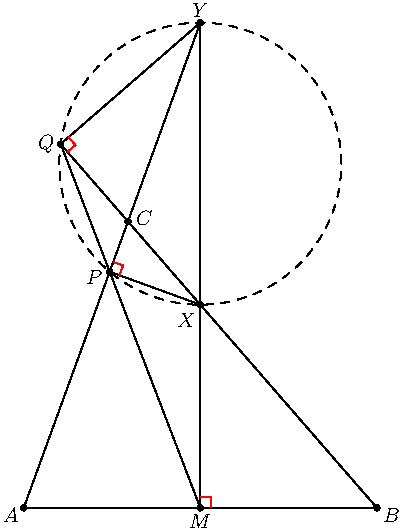
\includegraphics{g2fig}
\end{center}

\bigskip

\textbf{Marking Scheme - Solution 1 et 2}

\begin{itemize}
    \item 1P: Reformuler l'énoncé avec des angles, en une affirmation du type :
    \begin{itemize}
        \item $\angle MPX+\angle XPQ=180^\circ$
        \item $\angle XQP=\angle XQM$
    \end{itemize}
    \item 3P: Montrer que $YQPX$, $YQMB$ ou $AMXP$ sont cycliques (2P pour un quadrilatère, 3P pour deux ou trois quadrilatères)
    \item 1P: Montrer que $\angle MAX=\angle MBX$, $\angle MAY=\angle MBY$ ou que $\angle MYA=\angle MYB$.
    \item 2P: Conclure.
\end{itemize}

\textbf{Marking Scheme - Solution 3}

\begin{itemize}
    \item 1P: Reformuler l'énoncé comme une égalité de type Ménélaüs.
    \item 1P: Montrer que $YQPX$ est cyclique.
    \item 2P: Montrer $PA\cdot AY=XB\cdot BQ$.
    \item 1P: Montrer $CX\cdot QC=CP\cdot YC$.
    \item 2P: Conclure.
\end{itemize}
}

\newpage

\item[\textbf{K1)}] 
\de{Wir betrachten ein weisses $5\times 5$-Quadrat bestehend aus $25$ Einheitsquadraten. Wie viele verschiedene Möglichkeiten gibt es, eines oder mehrere der Einheitsquadrate schwarz anzumalen, sodass die resultierende schwarze Fläche ein Rechteck bildet?

\textbf{Lösung 1 (Tanish), Gegenüberliegende Ecken zählen}: Wir betrachten die Ecken eines beliebigen Rechtecks. Diese liegen in einem Raster bestehend aus $36$ Punkten in einem $6\times 6$ Quadrat. Wir wählen einen dieser Punkte als den ersten Eckpunkt. Wenn wir nun den gegenüberliegenden Eckpunkt wählen, haben wir ein Rechteck definiert. Gegenüberliegende Ecken können nicht in der selben Zeile oder Spalte liegen, wir wählen also einen von $25$ anderen Punkten. Total haben wir also $36$ mal $25$ Rechtecke. Aber wir haben jedes Rechteck $4$ mal gezählt - es gibt zwei Paare von gegenüberliegenden Ecken, die wir jeweils doppelt gezählt haben - wir teilen also unser Resultat durch $4$ und erhalten $9 \times 25 = 225$.
\newline
\textbf{Anmerkung (Jana)}: Es  ist auch möglich die möglichen Paare von gegenüberliegenden Eckpunkten folgendermassen zu zählen: Zuerst wählen wir zwei unterschidliche Punkte aus dem $6\times6$ Quadrat. Dafür gibt es $\binom{36}{2} = 18 \cdot 35$ Möglichkeiten. Jetzt müssen wir die Paare subtrahieren, welche sich in der gleichen Zeile oder Spalte befinden. Da es insgesamt $6$ Zeilen und $6$ Spalten gibt und wir in jeder dieser Spalten oder Zeilen $\binom{6}{2}$ Möglichkeiten haben ein Paar auszuwählen, müssen wir $12 \cdot \binom{6}{2} = 12 \cdot 15$ subtrahieren. In diesem Fall haben wir jedes Rechteck doppelt gezählt, wir erhalten also das Resultat $\frac{1}{2} \cdot (18 \cdot 35 - 12 \cdot 15) = 225$.


\textbf{Lösung 2 (Tanish), Zählen nach Höhe und Breite}: Wir betrachten die möglichen Rechtecke mit Höhe $a$ und Breite $b$. Das Einheitsquadrat oben links in unserem Rechteck liegt im \newline $(6-a) \times (6-b)$ Rechteck in der Ecke oben links in unserem grossen Quadrat, da unser Rechteck sonst keinen Platz hat. Die totale Anzahl Möglichkeiten ist also
\begin{align*}
    \sum_{a=1}^5 (6-a) \sum_{b=1}^5 (6-b) = \sum_{a=1}^5 (6-a)\cdot15 = 15\cdot15 = 225
\end{align*}
Analog hätten wir auch jeden anderen Eckpunkt unseres Rechtecks betrachten können.

\textbf{Lösung 3 (Tanish), Zählen nach Seiten}: Unser Rechteck ist eindeutig definiert durch ein Zeilen- und ein Spaltenpaar unseres Rasters (die zwei Zeilen und Spalten repräsentieren jeweils die obere und untere, respektive linke und rechte Seite unseres Rechtecks). Da wir aus $6$ Zeilen und $6$ Spalten wählen, haben wir total $\binom{6}{2}\cdot\binom{6}{2}=15^2=225$
Möglichkeiten.

\textbf{Lösung 4 (Tanish), Zählen nach beliebigem Eckpunkt}: Wir nummerieren unsere Einheitsquadrate mit $(x, y)$, wobei $(1,1)$ das Quadrat links unten und $(5,5)$ das Quadrat oben rechts ist. Wir betrachten nun alle Rechtecke, deren Eckfeld oben rechts $(a, b)$ ist. Das Rechteck ist einmalig definiert durch zwei gegenüberliegende Ecken, also müssen wir nur den gegenüberliegenden Eckpunkt $(<a, <b)$ wählen. Für dies gibt es $a \cdot b$ Möglichkeiten. Wenn wir über alle möglichen $(a, b)$ summieren, erhalten wir
\begin{align*}
    \sum_{a=1}^5 a \sum_{b=1}^5 b = \sum_{a=1}^5 a \cdot 15 = 15\cdot15 = 225
\end{align*}
Analog kann man auch jeden anderen Eckpunkt betrachten.

\textbf{Lösung 5 (Tanish), Zählen nach kürzester Seite}: Wir zählen alle Rechtecke mit kürzester Seite $x$. Nach der Ein-Ausschaltformel ist dies die Anzahl Rechtecke mit Höhe $x$ und Breite $\geq x$ plus die Anzahl Rechtecke mit Breite $x$ und Höhe $\geq x$ minus die Anzahl Rechtecke mit Breite \emph{und} Höhe $x$. Das Resultat in \emph{Lösung 2} zeigt, dass die Anzahl Rechtecke mit Dimensionen $a \times b$ durch $(6-a) \cdot (6-b)$ gegeben ist. Somit erhalten wir
\begin{align*}
    \sum_{x=1}^5 \bigg{(}( 2\cdot\sum_{y=x}^5 \bigg{(}(6-y)\cdot(6-x)\bigg{)} - (6-x)(6-x) \bigg{)} &= \sum_{x=1}^5 (6-x)(1 + 2 + \hdots (6-x) \hdots ... + 2 + 1) 
    \\ &= \sum_{x=1}^5 (6-x)(6-x)^2 
    \\ &= \sum_{x=1}^5 (6-x)^3 
    \\ &= 125 + 64 + 27 + 8 + 1 = 225
\end{align*}

Alle oben genannten Lösungen kann man für ein $n \times n$-Quadrat verallgemeinern.

\newpage

%\textbf{Marking Scheme}

%\begin{itemize}
  %  \item 1P: 225 als Antwort gegeben.
%\end{itemize}

  %  Wertvolle Bemerkungen (nicht additiv): 
  
%\begin{itemize}

    %\item +1P: Jegliche Versuche die Quadrate zu nummerieren (z.B. Koordinaten).
    
    %\item +2P: Jeglicher Versuch induktiv zu beweisen, dass die Anzahl Rechtecke um $n^3$ steigt, wenn man vom Fall $n-1$ zum Fall $n$ geht. +4P Ansonsten falls gezeigt wird, dass die Anzahl vom Fall $4 \times 4$ zu $5 \times 5$ um 125 ansteigt.

    %\item +3P: Behauptung, dass die Anzahl Rechtecke mit Dimensionen $a \times b$ durch $(6-a) \cdot (6-b)$ gegeben ist. +4P Ansonsten falls bemerkt wird, dass die Summe dieser Terme über $a, b$ das selbe ist wie die Summe von $ab$ über $a, b$.
    
   % \item +4P: Behauptung, dass ein Rechteck einmalig durch die Eckpunkte oben rechts und unten links oder durch die Eckpunkte oben links und unten rechts definiert ist. +5P falls ausserdem bemerkt wird, dass die Anzahl Möglichkeiten für den ersten Eckpunkt $ab$ ist. 
    
    %\item +4P: Behauptung, dass ein Rechteck einmalig durch ein geordnetes Paar von gegenüberliegenden Eckpunkten definiert ist \emph{und} das dies jedes Rechteck $4$ mal zählt (+2P falls dies vergessen wird). +5P Ansonsten falls ausserdem bemerkt wird, dass die Anzahl Möglichkeiten für die gegenüberliegende Ecke $25$ ist.
    
    %\item +5P: Behauptung, dass jedes Rechteck durch ein Paar von Zeilen und ein Paar von Spalten definiert ist (+4P falls anstatt $6$ Zeilen/Spalten $5$ gezählt werden)
    
    %\item +4P: Jegliche andere Summen, die nicht berechnet wurde, jedoch die korrekte Lösung $225$ ergibt.
    
    %\item +2P: Jegliche Summen, welche nicht $225$ ergeben, da sie gewisse Spezialfälle vergessen. (z.B. falls eine Methode nicht alle Rechtecke doppelt oder vierfach zählt, jedoch als solche betrachtet wird)
    
    %\item +6P: Jegliche korrekt berechnete \emph{und} begründete Summe.
    
%\end{itemize}

%Um die volle Punktzahl zu erreichen wird erwartet, dass nicht triviale Summen begründet werden.

\textbf{Marking scheme}%(Jana's Version)
\begin{itemize}
    \item 1P: Richtige Lösung $225$ (wird zu den restlichen Punkten addiert)
\end{itemize}
Die folgenden Punkte sind nicht additiv.
\begin{itemize}
    \item 1P: Quadrate irgendwie nummerieren oder die Rechtecke in disjunkte Gruppen aufteilen.
    \item 3P: Beobachtung, wie die Rechtecke gegeben sein können. (z.B. Auswahl gegenüberliegender Eckpunkte, ein Paar von Zeilen und ein Paar von Spalten)
    \item 4P: Begründete Summe, welche jedes Rechteck gleich oft zählt.
    \item 4P: Die Rechtecke in disjunkte Gruppen aufteilen und die Anzahl Rechtecke in jeder Gruppe berechnen.
    \item 5P: Begründete Formel, welche die Anzahl Rechtecke zählt
    %\item -2P: Fälle vergessen, sodass die Formel nicht alle Rechtecke gleich oft zählt
\end{itemize}

Ohne korrekte Formel sind maximum 4 Punkte möglich. Um die volle Punktzahl zu erreichen wird erwartet, dass nicht triviale Summen begründet werden.
}

\fr{On considère un carré blanc $5 \times 5$ composé de $25$ carrés unité. De combien de manières différentes peut-on colorier un ou plusieurs carrés unité en noir de telle manière que la surface noire obtenue soit un rectangle?

\textbf{Solution 1 (Tanish), Compter les sommets opposés}: On considère les sommets d'un rectangle quelconque. Ils sont situés sur une grille, qui est un groupe de 36 points dans un carré $6\times 6$. On choisit un de ces points comme premier sommet de notre rectangle. Si maintenant on choisit le sommet opposé, alors la paire formée par ces deux points suffit à définir le rectangle. Le sommet opposé ne peut pas être dans la même ligne ni dans la même colonne, donc est choisi parmi les 25 points restants. En répétant le calcul pour tous les 36 points, on a $36\times 25$ paires de points. Cependant on a compté chaque rectangle 4 fois - il y a deux paires différentes de sommets opposés, qui ont chacune été comptées deux fois (ce sont des paires ordonnées) - il faut donc diviser notre produit par 4 pour obtenir $9\times 25 = 225$.
\newline
\textbf{Remarque (Jana)}: Il est également possible de compter les choix possibles pour les sommets opposés de la manière suivante: on choisit d'abord deux points distincts dans la grille $6\times 6$. Il y a $\binom{36}{2} = 18 \cdot 35$ possibilités différentes. Ensuite il faut soustraire celles où les deux points sont situés sur la même ligne ou la même colonne. Puisqu'il y a $6$ lignes et $6$ colonnes et que dans les deux cas on a $\binom{6}{2}$ choix possibles, le nombre qu'il faut soustraire est $12 \cdot \binom{6}{2} = 12 \cdot 15$. On remarque encore qu'en procédant ainsi chaque rectangle est compté deux fois, donc le résultat final est $\frac{1}{2} \cdot (18 \cdot 35 - 12 \cdot 15) = 225$.

\textbf{Solution 2 (Tanish), Compter par hauteur et largeur}: On considère le nombre de rectangles possibles de dimension $a  \times b$, où $a$ est la hauteur et $b$ la largeur. Le carré en haut à gauche peut être n'importe quel carré du rectangle $(6-a) \times (6-b)$ placé en haut à gauche de la grille, car autrement le rectangle ne sera pas entièrement contenu dans le carré. Ainsi le nombre total de possibilités est
\begin{align*}
    \sum_{a=1}^5 (6-a) \sum_{b=1}^5 (6-b) = \sum_{a=1}^5 (6-a)\cdot15 = 15\cdot15 = 225
\end{align*}
De manière symétrique, on peut aussi considérer les positions possibles du carré en haut à droite, en bas à gauche ou en bas à droite en fonction des dimensions du rectangle.

\textbf{Solution 3 (Tanish), Compter par lignes/colonnes des côtés}: Notre rectangle est déterminé par le choix de deux lignes et deux colonnes sur la grille (les lignes représentent les côtés horizontaux et les colonnes représentent les côtés verticaux). On peut choisir parmi $6$ lignes et $6$ colonnes, donc le nombre total de possibilités est $\binom{6}{2}\cdot\binom{6}{2}=15^2=225.$

\textbf{Solution 4 (Tanish), Compter par le carré en haut à droite}: On numérote nos carrés avec les coordonnées $(x, y)$, avec $(1,1)$ désignant le carré en bas à gauche et $(5, 5)$ le carré en haut à droite. Maintenant regardons tous les rectangles dont le coin en haut à droite est $(a, b)$. Le rectangle est défini par le choix de son carré en haut à droite et de son carré en bas à gauche, donc il suffit de choisir un autre carré $(\leq a, \leq b)$, ce qui donne $a \cdot b$ possibilités. Par conséquent, en additionnant le nombre de possibilités pour tous les $(a, b)$ possibles, on obtient
\begin{align*}
    \sum_{a=1}^5 a \sum_{b=1}^5 b = \sum_{a=1}^5 a \cdot 15 = 15\cdot15 = 225
\end{align*}
De manière symétrique, cette preuve fonctionne aussi en considérant le carré en haut à gauche, en bas à droite ou en bas à gauche.

\textbf{Solution 5 (Tanish), Compter par le petit côté}: On compte tous les rectangles dont le petit côté a pour longueur $x$. Le principe d'inclusion-exclusion nous dit qu'il faut compter le nombres de rectangles de hauteur $x$ et de largeur $\geq x$ plus le nombre de rectangles de largeur $x$ et de hauteur $\geq x$ moins le nombre de rectangles de largeur \emph{et} de hauteur $x$. Par le résultat de la deuxième solution on sait déjà que le nombre de rectangles de dimension $a\times b$ est $(6-a)\cdot (6-b)$, donc on a
\begin{align*}
    \sum_{x=1}^5 \bigg{(}( 2\cdot\sum_{y=x}^5 \bigg{(}(6-y)\cdot(6-x)\bigg{)} - (6-x)(6-x) \bigg{)} &= \sum_{x=1}^5 (6-x)(1 + 2 + \hdots (6-x) \hdots ... + 2 + 1) 
    \\ &= \sum_{x=1}^5 (6-x)(6-x)^2 
    \\ &= \sum_{x=1}^5 (6-x)^3 
    \\ &= 125 + 64 + 27 + 8 + 1 = 225
\end{align*}

Les 5 solutions ci-dessus peuvent être généralisées au cas d'un carré $n\times n$.

\newpage

\textbf{Marking scheme}%(Jana's Version)
\begin{itemize}
    \item 1P: Affirmer que la réponse est $225$ (ce point peut être additionné aux autres points ci-dessous)
\end{itemize}
Les points ci-dessous sont non-additifs.
\begin{itemize}
    \item 1P: énumérer les carrés (p. ex. mettre des coordonnés) ou séparer les rectangles en ensembles disjoints.
    \item 3P: Trouver une manière de décrire chaque rectangle de manière unique (p. ex. en choisissant des sommets opposés, en choisissant lignes et colonnes, en choisissant la position du coin en haut à droite et les longueurs des côtés etc.)
    \item 4P: Formule qui compte chaque rectangle le même nombre de fois, avec justification. 
    \item 4P: Séparer les rectangles en ensembles disjoints et compter le nombre de rectangles dans chaque ensemble.
    \item 5P: Formule qui compte le nombre exact de rectangles, avec justification.
\end{itemize} 

Sans formule correct, au plus 4 points pourront être obtenus. Si des sommes non-triviales ne sont pas calculées explicitement il ne sera pas possible d'obtenir les 7 points.}

\en{Consider a white $5 \times 5$ square composed of $25$ unit squares. How many different ways are there to colour one or more unit squares black such that the resulting black area is a rectangle?

\textbf{Solution 1 (Tanish), Counting by opposite vertices}: Let us consider the possible vertices of any rectangle we create in the grid, which is the group of 36 points in a $6 \times 6$ square. Choose one of these as the first vertex of our rectangle. If we now choose the opposite corner, then the pair of these two points sufficiently define the rectangle. The opposite corner cannot be in the same column or line, so is one of 25 other points. Counting over all 36 points, we have $36 \times 25$ pairs of points. But we have counted each rectangle 4 times - there are two different pairs of opposite vertices which we each counted twice (they are ordered pairs) - so we divide our product by 4 to obtain $9 \times 25 = 225$.
\newline
\textbf{Remark (Jana)}: It's also possible to count the possible choices of opposite vertices in the following way: First we choose two distinct points in the $6\times6$-grid. There are $\binom{36}{2} = 18 \cdot 35$ possibilities to do that. Next we have to subtract those where both points lie in the same row or column. Since there are $6$ rows and $6$ columns and for each one we have $\binom{6}{2}$ possible choices, the number we subtract is $12 \cdot \binom{6}{2} = 12 \cdot 15$. Noticing that this way, each proper rectangle is counted twice, we obtain our final result $\frac{1}{2} \cdot (18 \cdot 35 - 12 \cdot 15) = 225$.

\textbf{Solution 2 (Tanish), Counting by height and width}: Let us consider the number of possible rectangles of dimension $a \times b$, where $a$ is the height and $b$ is the width. The top-left square can be any of the squares in a $(6-a) \times (6-b)$ rectangle in the top left, as otherwise the rectangle will not be fully contained in the square. Therefore the number of possibilities is
\begin{align*}
    \sum_{a=1}^5 (6-a) \sum_{b=1}^5 (6-b) = \sum_{a=1}^5 (6-a)\cdot15 = 15\cdot15 = 225
\end{align*}
Symmetrically, you could also have considered the possible locations of the top-right, bottom-left or bottom-right square in terms of the dimensions of the rectangle.

\textbf{Solution 3 (Tanish), Counting by rows/columns of sides}: Our rectangle is well defined by the choice of two rows and two columns of the grid (the rows representing the top and bottom side and the columns representing the left and right side). We have 6 rows and 6 columns to choose from, so the total number of possibilities is $\binom{6}{2}\cdot\binom{6}{2}=15^2=225.$

\textbf{Solution 4 (Tanish), Counting by top-right square}: Let us number our squares with coordinates $(x, y)$, with $(1,1)$ being the bottom-left square and $(5,5)$ the top-right square. Now let us look at all the rectangles whose top right corner is $(a, b)$. The rectangle is well-defined by the choice of a top-right and bottom-left square, so all we have to do is choose another square  $(<a, <b)$, of which there are $a \cdot b$ possibilities. Therefore, summing over all possible $(a, b)$ we have
\begin{align*}
    \sum_{a=1}^5 a \sum_{b=1}^5 b = \sum_{a=1}^5 a \cdot 15 = 15\cdot15 = 225
\end{align*}
Symmetrically, this proof also works when considering the top-left, bottom-right or bottom-left square.

\textbf{Solution 5 (Tanish), Counting by smallest side}: Let us count all the rectangles whose smaller side is of length $x$. Inclusion-Exclusion tells us that we should count the number of rectangles of height $x$ and width $\geq x$ plus the number of width $x$ and height $\geq x$ minus the number of width \emph{and} height $x$. By the result in proof 2 we already know the number of rectangles of dimension $a \times b$ is $(6-a) \cdot (6-b)$ so we have
\begin{align*}
    \sum_{x=1}^5 \bigg{(}( 2\cdot\sum_{y=x}^5 \bigg{(}(6-y)\cdot(6-x)\bigg{)} - (6-x)(6-x) \bigg{)} &= \sum_{x=1}^5 (6-x)(1 + 2 + \hdots (6-x) \hdots ... + 2 + 1) 
    \\ &= \sum_{x=1}^5 (6-x)(6-x)^2 
    \\ &= \sum_{x=1}^5 (6-x)^3 
    \\ &= 125 + 64 + 27 + 8 + 1 = 225
\end{align*}

All 5 of the proofs above can be generalised to an $n \times n$ square. 

\newpage

\textbf{Marking scheme}%(Jana's Version)
\begin{itemize}
    \item 1P: State the right answer $225$ (this can be added to the other marks)
\end{itemize}
The following are non-additive.
\begin{itemize}
    \item 1P: Any sensible attempt to enumerate the squares (e.g coordinates) or seperating the rectangles into disjoint sets.
    \item 3P: Finding a way of uniquely describing a rectangle (e.g by choosing opposite vertices, rows and columns, position of top right square and side lengths etc.)
    \item 4P: Justified expression that counts each rectangle the same number of times.
    \item 4P: Separating the rectangles into disjoint sets and counting the number of rectangles in each set.
    \item 5P: Justified formula for the exact number of rectangles
\end{itemize} 

Without a correct formula, at most 4 points can be awarded. To obtain full mark, non-trivial sums must be explicitely computed.

%\textbf{Marking Scheme}

%\begin{itemize}
   % \item 1P: State the answer 225.
%\end{itemize}

 %   Observations worth points (non-additive between themselves): 
  
%\begin{itemize}

    %\item +1P: Any attempt to enumerate the squares (e.g. coordinates).
    
    %\item +2P: Any attempt to inductively prove that the number of rectangles increases by $n^3$ when passing from the case $n-1$ to $n$. +4P instead if they also manage to prove that the increase from the case $4 \times 4$ to $5 \times 5$ is 125.

    %\item +3P: State that there are the number of rectangles of dimension $a \times b$ is $(6-a) \cdot (6-b)$. +4P instead if they remark that summing this product over all possible $a, b$ is the same thing as summing $ab$ over all possible $a, b$.
    
    %\item +4P: State that the rectangle is well-defined by the choice of a square in the top-right corner and a square in the bottom left corner. +5P instead if they also see that the number of possibilities for a given top corner is $ab$. 
    
    %\item +4P: State that the rectangle is well-defined by the choice of (ordered) opposite vertices \emph{and} that this counts every rectangle four times over (+2P instead if they forget to divide by four). Stating that using unordered pairs and dividing by 2 is also worth 4 points. +5P instead if they also see that the number of possible opposite corners for a given point is always 25. 
    
    %\item +5P: State that the rectangle is well-defined by the choice of two lines and two columns (+4P instead if they count 5 columns instead of 6)
    
    %\item +4P: Any other summation that they did not manage to compute, correctly justified, which when computed gives 225. 
    
    %\item +2P: Any summation which does not give 225 because it does not work for edge cases (for example, saying the rectangle is defined by the choice of a two opposite-corner squares, calculating the number of such pairs ($25 \cdot 24$), and dividing by 4 to give
    %150. This is incorrect because if the rectangle has a side of length 1 it is not counted 4 times over but just 2 times or once.)
    
    %\item +6P: Any correctly computed \emph{and} correctly justified summation.
    
%\end{itemize}
%Note that if the summation is too complicated then the contestant should justify why it is equal to 225 to get full marks (for instance, the summation in the fifth solution).
}

\newpage

\textbf{Alternative solutions}

\textbf{Solution 6 (Tanish), General proof by induction using bijections}: Let us prove the general result that the number of rectangles in a $n \times n$ square is $\sum_{i=1}^n i^3$. For the base case, there is clearly only 1 possible rectangle in a $1 \times 1$ square. Now suppose the proposition holds true for the case $n$. Now expand the grid to an $(n+1)\times(n+1)$ grid by adding a column on the right and a row on top. For every rectangle possible in the case $n$ we now modify it by moving its top-right corner one column up and to the right. This application represents a bijection between the rectangles in the case $n$ and the rectangles in the case $n+1$ without a side of length 1 (this can be verified by seeing that both the application and its inverse are surjective). It remains to count the "new" rectangles, or those with at least one side of length 1. These are well-defined by the choice of a square and then a square in the same row or column to represent the "ends" of the rectangle (the second square can be the same as the first one!), and this method counts every rectangle twice. We have $n^2$ choices for the first square and $2n$ choices for the second square after that ($n$ in the same row, $n$ in the same column) giving a total of $2n^3$ new rectangles, which we divide by 2, to give $n^3$. \\
\emph{Note:} It is possible to use this same method for solution 5 to count the number of rectangles of smaller side $x$, as these rectangles are well defined by the choice of two $x \times x$ squares in the same columns or rows (again, counting each rectangle twice).
\newpage

\item[\textbf{K2)}] 

\de{Das Dorf Roche hat $2020$ Einwohner. Eines Tages macht der berühmte Mathematiker Georges de Rham die folgenden Beobachtungen:
\begin{itemize}
    \item Jeder Dorfbewohner kennt einen weiteren mit dem gleichen Alter.
    \item In jeder Gruppe von $192$ Personen aus dem Dorf gibt es mindestens drei mit demselben Alter.
\end{itemize}{}
Zeige, dass es eine Gruppe von $22$ Dorfbewohnern gibt, die alle dasselbe Alter haben.

\textbf{Lösung:} Wir beweisen, dass höchstens $95$ verschiedene Alter vorkommen. Nehme an es treten $96$ oder mehr verschiedene Alter auf. Da jeder Dorfbewohner einen mit dem selben Alter kennt, können wir Paare mit $96$ verschiedenen Altern bilden, total gibt es also eine Gruppe von $192$ Dorfbewohnern, in welchen keine drei Personen das selbe Alter haben. Dies widerspricht de Rham's zweiter Bedingung. Da wir nun wissen, dass es höchstens $95$ verschiedene Alter gibt, können wir das Schubfachprinzip anwenden und sehen, dass mindestens eine Altersgruppe von mindestens $\lceil \frac{2020}{95} \rceil = 22$ Dorfbewohnern repräsentiert wird. Bemerke, dass $96$ verschiedene Alter zum selben Resultat führen, die stärkste Bedingung also $194$ anstatt $192$ ist.

\textbf{Marking Scheme:}
Die ersten beiden Punkte sind nicht additiv.
\begin{itemize}
    \item 2P: Beweis, dass die Aussage stimmt, falls es höchstens $k$ verschiedene Altersgruppen gibt für ein $k \in \{95,96 \}$ 
    \item 1P: Beweis, dass die Aussage stimmt, falls es höchstens $k$ verschiedene Altersgruppen gibt für ein $k \in \{92,93,94 \}$
    \item 5P: Beweis dafür, dass es höchstens $k$ Altersgruppen gibt für ein $k \in \{95,96 \}$

\end{itemize}
}

\fr{Dans le village Roche vivent 2020 personnes. Un jour, le fameux mathématicien Georges de Rham fait les observations suivantes:
\begin{itemize}
    \item Chaque villageois connaît un autre villageois du même âge que lui.
    \item Chaque groupe de 192 personnes dans le village contient toujours au moins trois personnes qui ont le même âge.
\end{itemize}
Montrer qu'il existe un groupe de 22 villageois qui ont tous le même âge.

\textbf{Solution:} On prouve qu'il y a au plus 95 âges différents: on suppose qu'il y plus de 96 âges différents. Comme chaque villageois connaît quelqu'un qui a le même âge que lui, on peut former un groupe de 192 villageois dans lequel on ne peut pas trouver un groupe de trois personnes qui ont le même âge. Cela contredit la deuxième hypothèse. Donc il existe au plus 95 âges différents. On applique le principe des tiroirs. Il existe un groupe d'âge dans lequel il y a au moins $\lceil \frac{2020}{95} \rceil = 22$ personnes.
Remarque: Ce résultat est aussi valable pour 96 âges différents, donc le cas maximal est un groupe de 194 personnes.

\textbf{Marking Scheme:}
Les deux premiers points ne sont pas additifs.
\begin{itemize}
    \item 2P: Montrer qu'il suffit de traiter le cas dans lequel il y a au plus $k$ âges différents, pour $k \in \{95,96 \}$ 
    \item 1P: Montrer qu'il suffit de traiter le cas dans lequel il y a au plus $k$ âges différents, pour $k \in \{92,93,94 \}$
    \item 5P: Montrer qu'il y a au plus $k$ âges différents, avec $k \in \{95,96 \}$

\end{itemize}


}

\ita{}

\en{The village of Roche has 2020 residents. One day, the famous mathematician Georges de Rham makes the following observations:
\begin{itemize}
  \item Every villager knows someone else with the same age as them.
  \item For any group of 192 people in the village, there are always at least three of them that have the same age.
\end{itemize}
Prove that there must exist a group of 22 villagers that all have the same age.

\textbf{Solution:} We prove there are at most 95 different possible ages. Suppose there are 96 or more different ages amongst them. Since each villager knows someone else with the same age as them, we can find two villagers for each of 96 different ages, forming a group of 192 villagers where no group of three with the same age exists, contradicting de Rham's second observation. Knowing that there are 95 different ages, we can now apply the pigeonhole principle to get that there is an age group represented at least $\lceil \frac{2020}{95} \rceil = 22$ times. Note that 96 different ages also yields this value, so the limiting case is groups of 194 people. 

\textbf{Marking Scheme:}
The first two are non-additive.
\begin{itemize}
    \item 2P: Show that it suffices to prove that there are at most $k$ different ages for some $k \in \{95,96 \}$ 
    \item 1P: Show that it suffices to prove that there are at most $k$ different ages for some $k \in \{92,93,94 \}$
    \item 5P: Prove that there are at most $k$ ages for some $k \in \{95,96 \}$

\end{itemize}
}





 

\newpage

\item[\textbf{Z1)}] 
\fr{Montrer que, pour tout nombre entier $n\geq 3$, il existe des nombres entiers strictement positifs $a_1<a_2<\ldots<a_n$ tels que
\[ a_k \div (a_1+a_2+\ldots+a_n) \]
pout tout $k=1,2,\ldots,n$.

\textbf{Solution 1:} La solution se fait par induction.
\begin{enumerate}
    \item Cas de base $n=3$: on observe que $1< 2< 3$ est une solution.
    \item Pas d'induction: soit $n \geq 4$ et supposons que le résultat soit vrai pour tout $m \leq n-1$. Soit $a_1<a_2<\ldots<a_{n-1}$ tels que $a_i \div \sum_{j=1}^n a_j$ pour tout $1 \leq i \leq n-1$. Alors, 
    \[
    a_1<a_2<\ldots<a_{n-1}<a_n:=\sum_{j=1}^{n-1}a_j
    \]
    vérifie aussi cette propriété. En effet, on observe tout d'abord que, comme $a_i>0$ pour tout $1 \leq i \leq n-1$, alors $a_n>a_{n-1}$. En outre, 
    \[
    \sum_{k=1}^n a_k=a_n+\sum_{j=1}^{n-1}a_j=2 \sum_{j=1}^{n-1}a_j.
    \]
    Par hypothèse de récurrence, $a_i \div 2\sum_{j=1}^{n-1}a_j=\sum_{k=1}^{n}a_k$ pour tout $1 \leq i \leq n-1$. De plus, $a_n=\sum_{j=1}^{n-1}a_j \div 2\sum_{j=1}^{n-1}a_j=\sum_{k=1}^n a_k$.
\end{enumerate}

%\textbf{Solution 1:} We will proceed by induction.
%\\Base case: $n=3$, 1, 2, 3 is a solution.
%\\Induction: Let $n \geq 4$ et assume that the statement holds for every $m \leq n-1$. Let $a_1<a_2<\ldots<a_{n-1}$ be such that $a_i \div \sum_{j=1}^n a_j \forall 1 \leq i \leq n-1$. Then $a_1,a_2,\ldots,a_{n-1},\sum_{j=1}^{n-1}a_j$ satisfy this property as well. Indeed $\sum_{k=1}^n a_k=\sum_{j=1}^{n-1}a_j+\sum_{k=1}^{n-1}a_k=2 \sum_{j=1}^{n-1}a_j$. By induction hypothesis $a_i \div 2\sum_{j=1}^{n-1}a_j=\sum_{k=1}^{n}a_k \forall 1 \leq i \leq n-1$. And $a_n=\sum_{j=1}^{n-1}a_j \div 2\sum_{j=1}^{n-1}a_j=\sum_{k=1}^n a_k$. Moreover since $a_i>0 \forall 1 \leq i \leq n-1, a_n>a_{n-1}$

\textbf{Solution 2:} On souhaite utiliser $\sum_{i=0}^n 2^i=2^{n+1}-1$. Observez que l'ensemble $1\leq 1< 2<\ldots<2^n$ vérifie la condition de divisibilité
\[
2^j \div (1+1+2+\ldots)=2^{n+1},\quad  \forall j=0,\ldots,n.
\]
Mais les nombres ne sont pas tous distincts. Pour construire une suite qui fonctionne, au lieu de considérer les puissances de 2, on considère les puissances de 2 multipliées par 3. La somme devient $\sum_{i=0}^n 3 \cdot 2^i=3 \sum_{i=0}^n 2^i=3 \cdot 2^{n+1}-3$. En ajoutant les nombres 1 et 2 aux puissances de 2 multipliées par 3, on trouve la solution: $1< 2< 3< 3 \cdot 2<\ldots< 3 \cdot 2^{n-3}$. En effet, la somme totale est $3\cdot 2^{n-2}$ et chaque nombre divise bien $3\cdot 2^{n-2}$.

%\textbf{Solution 2:} Since $\sum_{i=0}^n 2^i=2^{n+1}$, the set $1, 1, 2,\ldots,2^n$ satisfy $2^j \div \sum_{i=1}^n 2^i \forall 0 \leq j \leq n$. But the integers are not distinct. Multiplying the powers of 2 by 3, $\sum_{i=0}^n 3 \cdots 2^i=3 \sum_{i=0}^n 2^i=3 \cdots 2^{n+1}-3$. Adding 1 and 2 to this set gives a solution: $1, 2, 3, 3 \cdots 2,\ldots, 3 \cdots 2^{n-3}$. Indeed, each of the $3\cdots2^i$ divides $1+2+3\sum_{j=0}^{n-3} 2^j=2^{n-2} \forall 1 \leq i\leq n$.

\textbf{Solution 3: Reformulation.}\\ Supposons que nous avaons un ensemble $a_1, a_2 \dots a_n$ vérifiant la condition du problème, et soient $b_i = \frac{1}{a_i}(\sum_{k=1}^n a_k)$. Nous avons alors que $b_1, b_2 \dots b_n$ sont des entiers distincts satisfaisant
\[
\frac{1}{b_1}+\frac{1}{b_2}+\dots+\frac{1}{b_n} = 1
\]
et que construire un ensemble de $b_i$ avec cette propriété est équivalent au problème originel. Il y a plusieurs façons de le faire: une induction fonctionnerait par exemple en prenant $\{2, 3, 6\}$ comme ensemble de base et pour passer de $n$ à $n+1$, on remplace $b_n$ par $b_n+1$ et $b_n^2+b_n$ (en utilisant que $\frac{1}{x}-\frac{1}{x+1} = \frac{1}{x(x+1)}$). \\
\emph{Cette induction donne en fait une construction complètement différente des deux premières; le cas de base est le même, mais à chaque fois qu'on augmente $n$ de $1$, on multiplie chaque élément de l'ensemble par $1 + \sum_{k=1}^n a_k$ et on remplace le plus petit élément, qui était $1$ et qui est devenu $1 + \sum_{k=1}^n a_k$, par $1$ et $\sum_{k=1}^n a_k$. Pour aller à $n=4$, par exemple, on multiplie l'ensemble originel $\{1, 2, 3\}$ par $7$ pour obtenir $\{7, 14, 21\}$, et on remplace finalement $7$ par $6$ et $1$.}

\bigskip

\textbf{Marking Scheme}

\textbf{Solution 1}
\begin{itemize}
\item 1P: Avoir l'idée de l'induction.
\item 1P: Calculer le cas de base.
\item 2P: Avoir l'idée du pas d'induction (ajouter la somme des éléments à l'ensemble).
\item 2P: Montrer que le nouvel ensemble satisfait la condition.
\item 1P: Terminer la preuve.
\end{itemize}
\textbf{Solution 2}
\begin{itemize}
\item 4P: Trouver une construction.
\item 2P: Prouver que la condition est alors satisfaite.
\item 1P: Terminer la preuve.
\end{itemize}
}

\en{
\textbf{Solution 1: Induction} 
\begin{enumerate}
    \item Base case $n=3$: we observe that $1< 2< 3$ is a solution.
    \item Inductive step: Let $n \geq 4$ and suppose that the hypothesis is true for $n-1$. Let $a_1<a_2<\ldots<a_{n-1}$ such that $a_i \div \sum_{j=1}^n a_j$ for all $1 \leq i \leq n-1$ be the construction for that case. Then, 
    \[
    a_1<a_2<\ldots<a_{n-1}<a_n:=\sum_{j=1}^{n-1}a_j
    \]
    also has the desired properties. Firstly, since $a_i>0$ for all $1 \leq i \leq n-1$, such that $a_n>a_{n-1}$. Furthermore, 
    \[
    \sum_{k=1}^n a_k=a_n+\sum_{j=1}^{n-1}a_j=2 \sum_{j=1}^{n-1}a_j.
    \]
    By our inductive hypothesis, $a_i \div 2\sum_{j=1}^{n-1}a_j=\sum_{k=1}^{n}a_k$ for all $1 \leq i \leq n-1$. Additionally, $a_n=\sum_{j=1}^{n-1}a_j \div 2\sum_{j=1}^{n-1}a_j=\sum_{k=1}^n a_k$.
\end{enumerate}

%\textbf{Solution 1:} We will proceed by induction.
%\\Base case: $n=3$, 1, 2, 3 is a solution.
%\\Induction: Let $n \geq 4$ et assume that the statement holds for every $m \leq n-1$. Let $a_1<a_2<\ldots<a_{n-1}$ be such that $a_i \div \sum_{j=1}^n a_j \forall 1 \leq i \leq n-1$. Then $a_1,a_2,\ldots,a_{n-1},\sum_{j=1}^{n-1}a_j$ satisfy this property as well. Indeed $\sum_{k=1}^n a_k=\sum_{j=1}^{n-1}a_j+\sum_{k=1}^{n-1}a_k=2 \sum_{j=1}^{n-1}a_j$. By induction hypothesis $a_i \div 2\sum_{j=1}^{n-1}a_j=\sum_{k=1}^{n}a_k \forall 1 \leq i \leq n-1$. And $a_n=\sum_{j=1}^{n-1}a_j \div 2\sum_{j=1}^{n-1}a_j=\sum_{k=1}^n a_k$. Moreover since $a_i>0 \forall 1 \leq i \leq n-1, a_n>a_{n-1}$

\textbf{Solution 2: Constructive.}\\ We would like to use $\sum_{i=0}^n 2^i=2^{n+1}-1$. Observe that the set $1\leq 1< 2<\ldots<2^n$ verifies the divisibility condition
\[
2^j \div (1+1+2+\ldots)=2^{n+1},\quad  \forall j=0,\ldots,n.
\]
However, the numbers are not all distinct. To construct the set we desire, let us therefore consider what happens when we take the powers of 2 multiplied by 3 instead. The total sum is $\sum_{i=0}^n 3 \cdot 2^i=3 \sum_{i=0}^n 2^i=3 \cdot 2^{n+1}-3$. Now if we add on the numbers 1 and 2, we have the following set, which gives us everything we want: $1< 2< 3< 3 \cdot 2<\ldots< 3 \cdot 2^{n-3}$. The total sum is $3\cdot 2^{n-2}$ and every number divides $3\cdot 2^{n-2}$.

\textbf{Solution 3: Reformulation.}\\ Suppose we have a set $a_1, a_2 \dots a_n$ verifying the condition, and let $b_i = \frac{1}{a_i}(\sum_{k=1}^n a_k)$. It follows that $b_1, b_2 \dots b_n$ are distinct integers satisfying 
\[
\frac{1}{b_1}+\frac{1}{b_2}+\dots+\frac{1}{b_n} = 1
\]
and that constructing a set of $b_i$ that do this is strictly equivalent to solving the original problem. There are many ways of constructing such a set: one method is induction; take as a base case $\{2, 3, 6\}$ and when passing from $n$ to $n+1$, replace $b_n$ with $b_n+1$ and $b_n^2+b_n$ (simply exploiting the fact that $\frac{1}{x}-\frac{1}{x+1} = \frac{1}{x(x+1)}$). \\
\emph{This induction actually provides a completely different set of $a_i$ from the one in the first two solutions; the base case is the same but now every time you increase $n$ by $1$, you multiply every element of your previous set by $1 + \sum_{k=1}^n a_k$ and then replace the smallest element, which was previously $1$ and is now $1 + \sum_{k=1}^n a_k$, with 1 and $\sum_{k=1}^n a_k$. When going to $n = 4$, for example, you multiply the original set $\{1, 2, 3\}$ by $7$ to obtain $\{7, 14, 21\}$, and then replace the $7$ with a $6$ and a $1$.}

\bigskip
\textbf{Marking Scheme}

\textbf{Solution 1}
\begin{itemize}
\item 1P: Have the idea of induction.
\item 1P: Calculate the base case.
\item 2P: Have the idea of the induction step (Add the sum to the previous set).
\item 2P: Prove that the  new set satisfies the condition.
\item 1P: Finish the proof.
\end{itemize}
\textbf{Solution 2}
\begin{itemize}
\item 4P: Find a construction.
\item 2P: Prove that the condition is satisfied.
\item 1P: Finish the proof.
\end{itemize}
}

\de{Beweise, dass es für jede natürliche Zahl $n\geq 3$ natürliche Zahlen $a_1<a_2<\ldots<a_n$ gibt, sodass
\[ a_k \div (a_1+a_2+\ldots+a_n) \]
für jedes $k=1,2,\ldots,n$ gilt.

\textbf{Lösung 1:} Es wird mit Induktion bewiesen.
\begin{enumerate}
    \item Induktionsanfang, $n=3$:\\
    Man bemerke, dass $1< 2< 3$ die gegebene Bedingung erfüllt. Somit ist die Aussage wahr für $n=3$.
    \item Induktionsschritt:\\
    Nach der Induktionsannahme ist die Aussage wahr für alle $m \le n-1$. Seien also $a_1<a_2<\dots < a_{n-1}$ positiv, sodass $a_k \div \sum_{i=1}^{n} a_i$ für alle $1\le k\le n$ gilt.Wähle dazu $a_n = \sum_{j=1}^{n-1} a_j$.\\
    Da $a_i$ für $1\le i < n-1$ strikt grösser als $0$ ist, gilt $a_n > a_{n-1}$ und somit ist
    \[a_1 < a_2 < \dots < a_{n-1} < a_n = \sum_{j=1}^{n-1} a_j\]
    Man bemerke weiter, dass 
    \[\sum_{i=1}^{n} a_i = a_n + \sum_{i=1}^{n-1} a_i = 2\sum_{i=1}^{n-1} a_i\]
    Nach der Induktionsannahme gilt nun $a_k \div 2\sum_{i=1}^{n} a_i = \sum_{i=1}^{n}$ für alle $1\le k \le n-1$. Zusätzlich gilt nun aber auch $a_n = \sum_{i=1}^{n-1} a_i\div 2\sum_{i=1}^{n-1} a_i = \sum_{i=1}^{n} a_i$.\\
    Es erfüllen also die gewählten $a_1<\dots < a_n$ die Bedingung und der Induktionsschritt ist beendet.
   
\end{enumerate}


\textbf{Lösung 2:} Da, $\sum_{i=0}^n 2^{i} = 2^{n+1}-1$ ist, würden $1\le 1<2\dots<2^n$ die Teilbarkeitsbedingung erfüllen.
\[2^j \div (1+1+2+\dots + 2^n) = 2^{n+1}, \; \forall 0\le j\le n.\]
Nun sind die Zahlen jedoch nicht paarweise verschieden. Wir wollen also eine ähnliche Menge mit paarweise verschiedenen Zahlen konstruieren. Man multipliziert dazu alle Zweierpotenzen mit $3$ und fügt zusätzlich noch $1$ und $2$ hinzu. Man findet also hierzu die Zahlen $a_1 = 1<2<3<2\cdot 3 < \cdots < 3\cdot2^{n-3} = a_n$. Und in der Tat erfüllen diese Zahlen auch die Bedingung, da $\sum_{i=0}^{n} a_i = 3\cdot 2^{n-2}$ durch alle $a_i$ Teilbar ist.

\textbf{Lösung 3 (Reformulation):} Nehme wir an, dass die Menge $a_1, a_2, \dots, a_n$ die Bedingung erfüllt und seien $b_i = \frac{1}{a_i}\left(\sum_{k=1}^n\right)$. Es folgt, dass $b_i$ verschiedene positive ganze Zahlen sind, für welche gilt:
\[
\frac{1}{b_1}+\frac{1}{b_2}+\dots+\frac{1}{b_n} = 1
\]
Es genügt nun  eine Konstruktion für solche $b_i$ zu finden. Es gibt mehrere Möglichkeiten eine soche Menge  zu konstruieren: eine davon wäre mit Induktion.\\
Wir nehmen als Induktionsanfang die Menge ${2,3,6}$ und wenn wir von $n$ nach $n+1$ gehen ersetzen wir einfach $b'_n$ mit $b_n+1$ und $b_n^2+b'_n$ (wobei wir einfach $\frac{1}{x}-\frac{1}{x+1} = \frac{1}{x(x+1)}$ benutzen). \\
\emph{Diese Induktion führt tatsächlich zu einer komplett anderen Menge $a_i$  als in den obigen zwei Lösungen; die Anfangsmenge ist die Selbe, doch jedesmal wenn n um $1$ erhöht wird, multiplizieren wir alle vorherigen Elemente mit  $1+ \sum_{k=1}^{n} a_k$ und ersetzen das jetzt kleinste Element $1+ \sum_{k=1}^{n} a_k$ mit $1$ und  $\sum_{k=1}^n$. Zum Beispiel von n=3 nach n=4  multiplizieren wir die Ursprünglich Menge ${1,2,3}$ mit 7 um die neue Menge ${7,14,21}$ zu erhalten. Zusatsätzlich wird dann noch $7$ mit $1$ und $6$ ersetzt.}


\textbf{Marking Scheme}

\textbf{Lösung 1}
\begin{itemize}
\item 1P: Idee für Induktion zu benutzen.
\item 1P: Induktionsanfang.
\item 2P: Idee für den Induktionsschritt.
\item 2P: Zeigen, dass die neu konstruierte Menge die Bedingung erfüllt.
\item 1P: Den Beweis vollenden.
\end{itemize}
\textbf{Lösung 2}
\begin{itemize}
\item 4P: Konstruktion finden.
\item 2P: Zeigen, dass die Bedinguneg für die konstruierte Menge erfüllt sind.
\item 1P: Den Beweis vollenden.
\end{itemize}
}



\newpage 

\item[\textbf{Z2)}]
\de{
Bestimme alle natürlichen Zahlen $n \geq 2$, sodass für jeden Teiler $d > 1$ von $n$
\[d^2+n \, \div \, n^2+d\]
gilt.

\textbf{Antwort:} $n$ erfüllt die Bedingung genau dann, wenn es eine Primzahl ist.

\textbf{Lösung:} Zuest bemerken wir, dass alle Primzahlen die Voraussetzung tatsächlich erfüllen: Wenn $n$ eine Primzahl ist, muss $d=n$ gelten. Für diese Wahl von $d$ gilt offensichtlich
\[n^2 + n \, \div \, n^2 + n. \]

Wenn nun $n$ keine Primzahl ist, finden wir $a,b > 1$, sodass $n=ab$ gilt. Nun können wir $d=a$ wählen und erhalten
\[
a^2 + ab \, \div \, (ab)^2 + a.
\]
Hier können wir beide Seiten durch $a$ teilen und erhalten die äquivalente Teilbarkeitsbedingung
\[
a+b \, \div \, ab^2 + 1.
\]
Analog dazu können wir auch $d=b$ wählen und erhalten
\[
b^2 + ab \, \div \, (ab)^2 + b \quad \Longleftrightarrow \quad b + a \, \div \, a^2b + 1.
\]
Wir sehen also, dass $a+b$ sowohl $ab^2+1$ als auch $ab^2+1$ teilt, also auch deren Summe:
\[
a+b \, \div \,  ab(a+b)+2.
\]
Offensichtlich ist $ab(a+b)$ durch $a+b$ teilbar. Dann sagt uns die obige Bedingung, dass
\[
a+b \, \div \, 2
\]
gilt. Dies steht aber im Widerspruch zu $a,b > 1$! Wir folgern also, dass alle nicht-Primzahlen die Bedingung der Aufgabe nicht erfüllen.

\textbf{Alternative:} Wir können auch die Differenz von $ab^2+1$ und $a^2b+1$ betrachten, woraus wir
\[a+b \div ab(a-b)\]
erhalten. Falls wir nun ggT$(a,b) = 1$ wählen können, würde dies ggT$(a+b,ab)=1$ und somit
\[a+b \div a-b\]
implizieren, was unmöglich ist.\\
Wir können $a$ und $b$ allerdings nur dann teilerfremd wählen, falls $n$ mindestens zwei verschiedene Primteiler hat. Wir müssen also den Fall, in dem $n$ eine Primpotenz ist, noch separat behandeln: \\
Falls $n= p^k$ für $p$ prim und $k\ge 2$, können wir aber einfach $d=p$ wählen um
\[
p^2 + p^k \, | \, p^{2k} + p \quad \Longrightarrow \quad p^2 \, | \, p\left(p^{2k-1}+1\right) \quad \Longrightarrow \quad p \, | \, p^{2k-1} + 1
\]
zu erhalten, was auch unmöglich ist.

\textbf{Marking scheme (Additiv)}
 \begin{itemize}
    \item 1P: Beobachtung, dass alle Primzahlen funktionieren
    \item 1P: Eine Teilbarkeitsbedingung der Form $a+b \, | \, ab^2 + 1$ für $n=ab$
    \item 2P: Die zweite Teilbarkeitsbedigung der Form $a+b \, | \, a^2b + 1$ für $n=ab$
    \item 2P: $a+b \, | \, a^2b + ab^2 + 2$ \textbf{oder} $a+b \, | \, ab(b-a)$ und den Fall $n=p^k$ ausschliessen
    \item 1P: Vervollständigung des Beweises
    \end{itemize}
}

\en{
Find all positive integers $n \geq 2$ such that, for every divisor $d> 1$ of $n$, we have
\[d^2+n \, \div \, n^2+d.\]

\textbf{Answer:} $n$ satisfies the condition of the problem if and only if it is a prime.

\textbf{Solution:} First we observe that all prime numbers satisfy the condition: If $n$ is a prime number, the only allowed value for $d$ is $d=n$ and plugging this into the divisibility condition, we get
\[n^2 + n \, \div \, n^2 + n, \]
which is obviously true.

Now, if $n$ is not a prime number, we can write $n=ab$, where $a$ and $b$ are integers greater than $1$. Assume that $n$ satisfies the conditions of the problem. If we choose $d=a$ and substitute $n=ab$ into the divisibility, we get
\[
a^2 + ab \, \div \, (ab)^2 + a.
\]
Observe that both sides are divisible by $a$, so we can divide both sides by $a$ to obtain the equivalent statement
\[
a + b \, \div ab^2 + 1.
\]
Analogously, if we choose $d=b$ instead, we get
\[
b^2 + ab \, \div \, (ab)^2 + b \quad \Longleftrightarrow \quad b + a \, \div \, a^2b + 1.
\]
Hence, we see that $a+b$ divides both the expressions $ab^2+1$ and $a^2b+1$, so it divides their sum as well:
\[
a+b \, \div \,  ab(a+b)+2.
\]
Since $ab(a+b)$ is obviously divisible by $a+b$, the above condition tells us
\[
a+b \, \div \, 2.
\]
However, since $a,b > 1$, we must have $a+b > 2$ and this is clearly a contradiction to the divisibility above. We conclude that therefore all non-primes cannot satisfy the condition of the problem.

\textbf{Alternative route:}
We can also take the difference of $a^2b+1$ and $ab^2+1$ to obtain
\[
a+b \, | \, ab(a-b).
\]
Now, if we could choose gcd$(a,b)=1$, this would also imply gcd$(a+b,ab)=1$, and hence 
\[
a+b \, | \, a-b,
\]
which is impossible. We can choose $a,b$ coprime if and only if $n$ has at least two different prime factors, so the case where $n$ is a prime power is not covered. However, if $n=p^k$ for some $k \geq 2$, we can choose $d=p$ and get 
\[
p^2 + p^k \, | \, p^{2k} + p \quad \Longrightarrow \quad p^2 \, | \, p(p^{2k-1}+1) \quad \Longrightarrow \quad p \, | \, p^{2k-1} + 1,
\]
which is clearly impossible.

\textbf{Marking scheme (additive)}
\begin{itemize}
    \item 1P: Stating that all primes work
    \item 1P: A divisibility condition of the form $a+b \, | \, ab^2 + 1$ for $n=ab$
    \item 2P: The second divisibility condition $a+b \, | \, a^2b + 1$ for $n=ab$
    \item 2P: $a+b \, | \, a^2b + ab^2 + 2$ \textbf{or} $a+b \, | \, ab(b-a)$ and excluding the case $n=p^k$
    \item 1P: Finishing the proof
\end{itemize}
}

\fr{
Trouver tous les nombres entiers $n \geq 2$ tels que tout diviseur $d > 1$ de $n$ vérifie
\[d^2+n \, \div \, n^2+d.\]

\textbf{Réponse:} $n$ satisfait la condition du problème si et seulement si c'est un nombre premier.

\textbf{Solution:} Tout d'abord nous observons que tous les nombres premiers satisfont la condition: Si $n$ est un nombre premier, la seule valeur que peut prendre $d$ est $d=n$ et en remplaçant dans l'équation on a besoin de 
\[n^2 + n \, \div \, n^2 + n, \]
qui est clairement vraie.

Maintenant, si $n$ n'est pas un nombre premier, on peut écrire $n=ab$, où $a$ et $b$ sont des entiers plus grands que $1$. Supposons que $n$ satisafait les conditions du problème. Si on choisit $d=a$ et on substitue $n=ab$ dans la divisibilité, on obtient
\[
a^2 + ab \, \div \, (ab)^2 + a.
\]
Observons que les deux côtés sont divisibles par $a$, et on peut diviser les deux par $a$ pour obtenir l'affirmation équivalente
\[
a + b \, \div ab^2 + 1.
\]
De façon analogue, en choisissant $d=b$, nous obtenons
\[
b^2 + ab \, \div \, (ab)^2 + b \quad \Longleftrightarrow \quad b + a \, \div \, a^2b + 1.
\]
Ainsi, nous voyons que $a+b$ divise les expressions $ab^2+1$ et $a^2b+1$, donc $a+b$ divise leur somme:
\[
a+b \, \div \,  ab(a+b)+2.
\]
Comme $ab(a+b)$ est clairement divisible par $a+b$, la condition du dessus nous donne
\[
a+b \, \div \, 2.
\]
Cependant, comme $a,b > 1$, nous avons $a+b > 2$, une contradiction avec la divisibilité plus haut. Nous concluons alors qu'aucun nombre composé (qui n'est pas premier) ne peut satisfaire la condition du problème.

\textbf{Route alternative:}
Nous pouvons aussi soustraire $ab^2+1$ de $a^2b+1$ et ainsi obtenir
\[
a+b \, | \, ab(a-b).
\]
Maintenant, si nous pouvions forcer pgdc$(a,b)=1$, cela impliquerait pgdc$(a+b,ab)=1$, et ainsi
\[
a+b \, | \, a-b,
\]
ce qui est impossible. On peut choisir $a, b$ premiers entre eux si et seulement si $n$ a au moins deux diviseurs premiers distincts, donc il nous manque juste le cas où $n$ est une puissance d'un premier. Or, si $n=p^k$ pour $k\geq 2$, nous pouvons choisir $d=p$ et obtenir
\[
p^2 + p^k \, | \, p^{2k} + p \quad \Longrightarrow \quad p^2 \, | \, p(p^{2k-1}+1) \quad \Longrightarrow \quad p \, | \, p^{2k-1} + 1,
\]
ce qui est clairement impossible.

\newpage

\textbf{Marking scheme (additif)}
\begin{itemize}
    \item 1P: Affirmer que tous les premiers fonctionnent.
    \item 1P: Une condition de divisibilité de la forme $a+b \, | \, ab^2 + 1$ pour $n=ab$.
    \item 2P: La seconde condition de divisibilité $a+b \, | \, a^2b + 1$ pour $n=ab$.
    \item 2P: $a+b \, | \, a^2b + ab^2 + 2$ \textbf{ou} $a+b \, | \, ab(b-a)$ et exclure le cas $n=p^k$.
    \item 1P: Terminer la preuve.
\end{itemize}
}

\end{enumerate}

\end{document}